\documentclass{article}

\usepackage{tikz}
\usepackage{stfloats}
\usetikzlibrary{arrows}
\usepackage{amsthm,amsmath,amssymb,natbib}
\usepackage{hyperref}
% For algorithms
\usepackage{algorithm}
\usepackage{algorithmic}
\usepackage{fancyvrb}
\usepackage{graphicx}

\usepackage{xcolor}
\definecolor{Ckt}{HTML}{E41A1C}
\definecolor{Min}{HTML}{4D4D4D}%grey30
%{B3B3B3}%grey70
\definecolor{MinMore}{HTML}{377EB8}
\definecolor{Data}{HTML}{984EA3}
\newtheorem{proposition}{Proposition}
\newtheorem{remark}{Remark}
\newtheorem{lemma}{Lemma}
\newtheorem{theorem}{Theorem}
\newtheorem{definition}{Definition}
\DeclareMathOperator*{\argmin}{arg\,min}
\DeclareMathOperator*{\sign}{sign}
\DeclareMathOperator*{\Lik}{Lik}
\DeclareMathOperator*{\Peaks}{Peaks}
\DeclareMathOperator*{\HotSpots}{HotSpots}
\newcommand{\Cost}{\text{Cost}}
\DeclareMathOperator*{\Diag}{Diag}
\DeclareMathOperator*{\TPR}{TPR}
\DeclareMathOperator*{\Segments}{Segments}
\DeclareMathOperator*{\Changes}{Changes}
\DeclareMathOperator*{\FPR}{FPR}
\DeclareMathOperator*{\argmax}{arg\,max}
\DeclareMathOperator*{\maximize}{maximize}
\DeclareMathOperator*{\minimize}{minimize}
\newcommand{\ZZ}{\mathbb Z}
\newcommand{\NN}{\mathbb N}
\newcommand{\RR}{\mathbb R}

\begin{document}

\title{A scalable machine learning pipeline for joint peak calling
  reveals differences between cell and experiment types}
\author{Toby Dylan Hocking and Guillaume Bourque}
\maketitle

\section{Results}

\begin{figure}
  \centering
  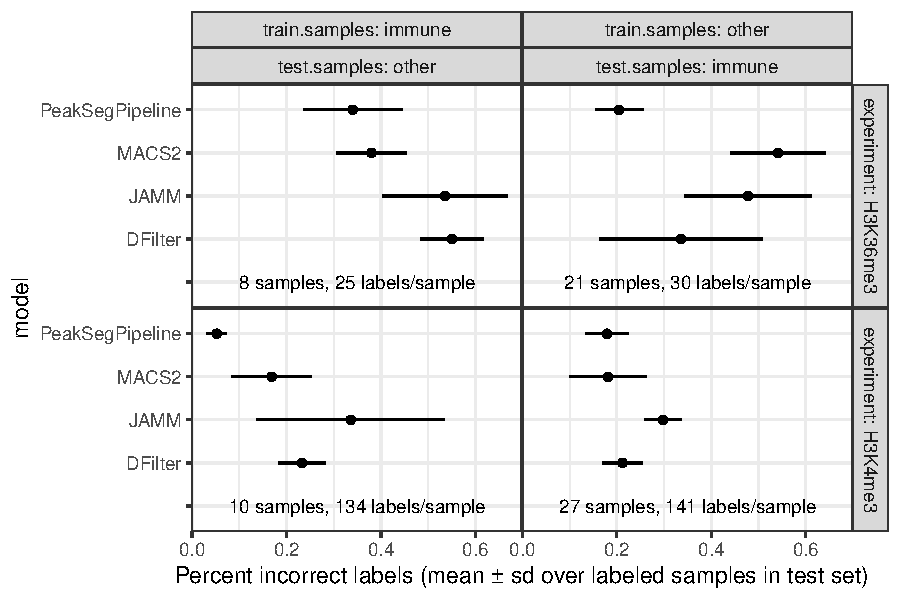
\includegraphics[width=\textwidth]{figure-test-error}
\end{figure}

\section{Time and memory requirements}

PeakSegPipeline uses algorithms with log-linear time complexity in the
number of samples and base pairs. The PeakSegFPOP algorithm for peak
prediction in a single sample with $n$ coverage data (lines in the
bedGraph file) uses $O(\log n)$ memory, $O(n \log n)$ disk space, and
$O(n\log n)$ time
\citep{Hocking-constrained-changepoint-detection}. In practice we
assign each job 10GB RAM and 24 hours of compute time. The total
pipeline takes several hours or days to run (depending on the number
of labels and samples).

PeakSegPipeline analyzes the data at single base pair resolution, and
has no arbitrary bin or window size parameters.

JAMM ran out of memory (over 20GB) when analyzing the tcell group, which
had the most samples (15 H3K36me3 tcell samples, 19 H3K4me3 tcell
samples). So for the tcell group we only used five samples, which took
16GB of RAM and 11-16 hours of compute time.

\bibliographystyle{abbrvnat}
\bibliography{refs}

\end{document}


